% mnras_template.tex
%
% LaTeX template for creating an MNRAS paper
%
% v3.0 released 14 May 2015
% (version numbers match those of mnras.cls)
%
% Copyright (C) Royal Astronomical Society 2015
% Authors:
% Keith T. Smith (Royal Astronomical Society)

% Change log
%
% v3.0 May 2015
%    Renamed to match the new package name
%    Version number matches mnras.cls
%    A few minor tweaks to wording
% v1.0 September 2013
%    Beta testing only - never publicly released
%    First version: a simple (ish) template for creating an MNRAS paper

%%%%%%%%%%%%%%%%%%%%%%%%%%%%%%%%%%%%%%%%%%%%%%%%%%
% Basic setup. Most papers should leave these options alone.
\documentclass[a4paper,fleqn,usenatbib]{mnras}

% MNRAS is set in Times font. If you don't have this installed (most LaTeX
% installations will be fine) or prefer the old Computer Modern fonts, comment
% out the following line
\usepackage{newtxtext,newtxmath}
% Depending on your LaTeX fonts installation, you might get better results with one of these:
%\usepackage{mathptmx}
%\usepackage{txfonts}

% Use vector fonts, so it zooms properly in on-screen viewing software
% Don't change these lines unless you know what you are doing
\usepackage[T1]{fontenc}
\usepackage{ae,aecompl}


%%%%% AUTHORS - PLACE YOUR OWN PACKAGES HERE %%%%%

% Only include extra packages if you really need them. Common packages are:
\usepackage{graphicx}	% Including figure files
\usepackage{amsmath}	% Advanced maths commands
\usepackage{amssymb}	% Extra maths symbols
\usepackage{deluxetable}


%%%%%%%%%%%%%%%%%%%%%%%%%%%%%%%%%%%%%%%%%%%%%%%%%%

%%%%% AUTHORS - PLACE YOUR OWN COMMANDS HERE %%%%%

% Please keep new commands to a minimum, and use \newcommand not \def to avoid
% overwriting existing commands. Example:
%\newcommand{\pcm}{\,cm$^{-2}$}	% per cm-squared

%%%%%%%%%%%%%%%%%%%%%%%%%%%%%%%%%%%%%%%%%%%%%%%%%%

%%%%%%%%%%%%%%%%%%% TITLE PAGE %%%%%%%%%%%%%%%%%%%

% Title of the paper, and the short title which is used in the headers.
% Keep the title short and informative.
\title[Mid--IR RR Lyrae PL Relation in $\omega$ Cen]{The Carnegie RR Lyrae Program: The Mid--Infrared RR Lyrae Period--Luminosity Relation in $\omega$ Centauri}

% The list of authors, and the short list which is used in the headers.
% If you need two or more lines of authors, add an extra line using \newauthor
\author[M. Durbin et al.]{
Meredith Durbin$^{1,2}$\thanks{E-mail: mdurbin@stsci.edu}
Victoria Scowcroft$^{3}$
Wendy Freedman$^{4}$
Gurtina Besla$^{5}$ 
\newauthor Giuseppe Bono$^{6, 7}$
Maria--Rosa Cioni$^{8, 9, 10}$
Gisella Glementini$^{11}$
Kathryn Johnston$^{12}$
\newauthor Nitya Kallivayalil$^{13}$
Juna Kollmeier$^{3}$
David Law$^{2}$
Barry Madore$^{3}$
Steve Majewski$^{13}$
\newauthor Roeland van der Marel$^{2}$
Massimo Marengo$^{14}$
Andrew~J.~Monson$^{3}$
David Nidever$^{15}$ 
\newauthor
Grzegorz Pietrzynski$^{16, 17}$
George Preston$^{3}$
Mark Seibert$^{3}$
Horace Smith$^{18}$
\newauthor Igor Soszynski$^{16}$
Ian Thompson$^{3}$
Andrzej Udalski$^{16}$
\\
% List of institutions
$^1$ Pomona College, Claremont, CA 91711, USA \\
$^2$ Space Telescope Science Institute, 3700 San Martin Drive, Baltimore, MD 21218, USA \\
$^3$ Observatories of the Carnegie Institution of Washington, 813 Santa Barbara St., Pasadena, CA 91101, USA \\
$^4$ Department of Astronomy and Astrophysics, University of Chicago, 5640 S Ellis Ave, Chicago, IL 60637, USA \\
$^5$ Department of Astronomy and Steward Observatory, University of Arizona, 933 North Cherry Avenue,   Tucson, AZ 85721, USA \\
$^6$ Univ. Roma ``Tor Vergata", Via della Ricerca Scientifica, 1 - 00133, Roma, Italy \\
$^7$ INAF-OAR, via Frascati 33 - 00040, Monte Porzio Catone (RM), Italy \\
$^8$ Universtat Potsdam, Institut fur Physik und Astronomie, Karl-Liebknecht-Str. 24/25, 14476 Potsdam, Germany \\
$^9$ Leibniz-Institut fur Astrophysik Potsdam, An der Sternwarte 16, 14482 Potsdam, Germany \\
$^{10}$ University of Hertfordshire, Physics, Astronomy and Mathematics, College Lane, Hatfield AL10 9AB, United Kingdom \\
$^{11}$ INAF - Osservatorio Astronomico, Via Ranzani n. 1, 40127 Bologna, Italy \\
$^{12}$ Department of Astronomy, Columbia University, New York, NY 10027, USA  \\
$^{13}$ Department of Astronomy, University of Virginia, Charlottesville, VA 22904-0818, USA \\
$^{14}$ Department of Physics and Astronomy, Iowa State University, Ames, IA, USA \\
$^{15}$ Department of Astronomy, University of Michigan, Ann Arbor, MI 48109, USA \\
$^{16}$ Warsaw University Observatory Al. Ujazdowskie 4, 00-478 Warszawa, Poland \\
$^{17}$ Departamento de Astronomia, Universidad de Concepcion, Casilla 160-C, Chile \\
$^{18}$ Department of Physics and Astronomy, Michigan State University, East Lansing, MI, USA 48824 \\
}

% These dates will be filled out by the publisher
\date{Accepted XXX. Received YYY; in original form ZZZ}

% Enter the current year, for the copyright statements etc.
\pubyear{2015}

% Don't change these lines
\begin{document}
\label{firstpage}
\pagerange{\pageref{firstpage}-\pageref{lastpage}}
\maketitle

% Abstract of the paper
\begin{abstract}
Something something metallicity
%We present new period-luminosity relations for RR Lyrae variables in 3.6 and 4.5 \micron\ derived from time-resolved IRAC data of $\omega$ Centauri. The sample consists of 36 RR Lyrae in 3.6 \micron\ and 37 in 4.5 \micron, 22 of which appear in both channels and have literature values for metallicities. We find no compelling evidence for a metallicity correlation in the residuals, based on a spread of 1.2 dex in [Fe/H].
\end{abstract}

% Select between one and six entries from the list of approved keywords.
% Don't make up new ones.
\begin{keywords}
keyword1 - keyword2 - keyword3
\end{keywords}

%%%%%%%%%%%%%%%%%%%%%%%%%%%%%%%%%%%%%%%%%%%%%%%%%%

%%%%%%%%%%%%%%%%% BODY OF PAPER %%%%%%%%%%%%%%%%%%

%% IMPORTANT NOTES FROM VS:

% MNRAS is a UK journal - change your spellcheck language in your editor to British English. 
% Correct plural of RR Lyrae is RR Lyrae variables (technically, singular should be RR Lyrae variable, as RR Lyrae itself is a named object)
% Use 1 dash - for a minus sign in math mode
% Use 2 dashes -- to hyphenate words
% Use 3 dahses --- to put a dash between parts of a sentence or to denote a minus sign outside of math mode
% Figures and tables can go at their appropriate places in the document rather than at the end. 
% To update bibtex source run ads_importer.py omegaCen_mnras_2015 after latex, then run latex, bibtex, latex, latex (ads_importer.py is available from VS's github, rely's on ADS style refs).


\section{Introduction}
\label{sec:intro}
The Carnegie Hubble Program (CHP) is a Warm \textit{Spitzer} program with the aim of measuring $H_{0}$ to a systematic uncertainty of 3\%, eventually reducing that uncertainty to 2\% using \textit{JWST}. The first part of the CHP used Cepheids as the primary distance indicator, using parallax measurements of Cepheids from \textit{HST} \citep{2007AJ....133.1810B} to calibrate the zero--point of the Cepheid Period--Luminosity (PL) relation (also known as the Leavitt Law, or LL), leading out to Cepheid measurements in the Milky Way \citep[MW,][]{2012ApJ...759..146M} and Large Magellanic Cloud \citep[LMC,][]{2011ApJ...743...76S}. An initial recalibration of $H_{0}$ from CHP was presented in \citet{2012ApJ...758...24F}.

The CHP removed many systematics from the $H_{0}$ measurement by moving to the mid--infrared (extinction is reduced by a factor of 16 to 20, amplitude of Cepheid pulsation is reduced, intrinsic width of LL is reduced) and by using a single instrument (no effects from ground--to--space transformation, for example) but there are some effects that cannot be accounted for without further tests. By only using a single distance indicator (i.e. Cepheids) for the zero--point measurement, we have no understanding of the intrinsic accuracy of our measurement. With recent measurements from cosmic microwave background (CMB) experiments such as Planck \citep{2015arXiv150201589P} in tension with local $H_{0}$ values, we must assess all possible sources of systematic uncertainty in our measurement. This is where the Carnegie RR Lyrae Program comes into play.

** VS NOTE: With regard to CMB - is measurements the correct word here? Obviously Planck et al. make measurements, but they do not measure $H_{0}$, it is inferred from a model. What word would be more appropriate here? **

The Carnegie RR Lyrae Program (CRRP) assess a systematic that was unreachable in the original CHP -- the intrinsic accuracy of the mid--infrared Cepheid standard candle distance scale when compared to the standard ruler distance scale of CMB and Baryon Acoustic Oscillation (BAO) measurements. With only one ``test candle'' it is impossible to make any assessment of this accuracy. However, when we have two standard candles with similar precision we can make meaningful comparisons and assess the systematic accuracy of both of them.

In the past RR Lyrae variables have often been thought of as the poor substitute for Cepheids in terms of distance scale measurements. They are intrinsically fainter, and in the optical follow a much shallower, even horizontal, PL relation. Determining an accurate distance to an RR Lyrae (RRL) in the $V$ band requires knowledge of its [Fe/H] -- a quantity which itself is not  easy to obtain. However, in more recent years near-- and mid--infrared observations have shown the true power of RRL as precision distance indicators. In a similar vein to Cepheids, \text{HST} parallaxes were obtained for several Galactic RRL calibrators \citet{2011AJ....142..187B} and several groups have been studying the populations of RRL in globular clusters and nearby dwarf spheroidal galaxies (NEED REFS). 

In the mid--infrared RRL exhibit similar properties to Cepheids\citep{2013ApJ...776..135M}. Their light curve amplitudes are minimised as we are seeing deeper into the star. At the wavelengths observed by Warm \textit{Spitzer} (3.6 and 4.5~$\mu$m) we do not see photospheric effects, but only the effects of temperature driving the pulsation. Essentially, the mid--infrared light curve is tracing the radius change of the star. A by--product of this effect is that the intrinsic width of the RRL PL relation is also minimised in the mid--infrared (mid--IR). The PL relation for pulsational variables can be thought of as a two--dimensional projection of the three--dimensional period--luminosity--colour relation (see figure 3 of \citet{1991PASP..103..933M} for a graphical representation). As the colour--width decreases in the mid--IR, the width of the PL naturally decreases. As one moves from the optical to the mid--IR, the slope of the PL relation steepens and its dispersion dramatically decreases; this phenomenon has been demonstrated in simulations by \citet{2004ApJS..154..633C}, and by several observational efforts, as illustrated in fig. 4 of \citet{2013ApJ...776..135M}. The slope should asymptotically approach the predicted slope of the period--radius relation, resulting in a slope between $-2.4$ and $-2.8$. Through this decrease in dispersion we have found that the intrinsic width of the mid--IR PL for RRL is in fact smaller than for Cepheids -- 0.05~mag compared to 0.10~mag (Monson et al. 2015, Neely et al. 2015). This translates to an uncertainty on an individual RR Lyrae star of 2\%, compared to 4\% for Cepheids. 

In this work we present the mid--IR PL relation for the RRL in the $\omega$~Cen Galactic Globular Cluster (GGC). 
Here we present a mid--infrared of the RR Lyrae period--luminosity (PL) relation in the IRAC channels 1 and 2 centred on 3.6 and 4.5 \micron\ respectively, as well as a preliminary investigation into metallicity effects on the PL relation.

There are very few metallic or molecular transition lines in the mid--IR at typical RR Lyrae temperatures, so the effects of metallicity on luminosity should be minimised. However, $\omega$~Cen provides the ideal test bed for any effect that we may not have predicted. Such an effect is not out of the realm of possibility; for example, the CO band head at 4.5~$\mu$m has been found to have a significant dependence on metallicity, and has such prevented the IRAC 4.5~$\mu$m Cepheid observations from being used for distance measurements in the CHP. As our concern in this program is systematic precision, we must ensure that similar effects do not plague the RRL distance scale.  

$\omega$ Cen in particular is ideal for calibrating the RR Lyrae period--luminosity--metallicity relation, as it contains 192 known RR Lyrae \citep{2004A&A...424.1101K} with a metallicity range spanning over 1.5 dex (Bono 2013, private communication); a metallicity spread this wide is not found in any other GGC. As noted in \citet{2006MNRAS.372.1675S}, one of the advantages of using globular clusters to calibrate PL coefficients is that all stars in a cluster can be considered to be at the same distance from Earth. We can therefore assume that any dispersion in the PL relation is a combination of the a) the intrinsic dispersion of the PL relation, b) the photometric uncertainties, and c) dispersion induced by the spread in metallicity of the RRL. We have measured the intrinsic dispersion of the RRL PL from other clusters (e.g. M4, Neely et al. 2015), and our photometric uncertainties are a well defined \textbf{constraint, value?? what is the correct word?}, so the only unknown in this problem is the dispersion due to the spread in metallicity of the cluster. We are lucky with $\omega$~Cen that we can also take a second approach to establishing the metallicity effect on the RRL PL relation. As it is such a unique object, $\omega$~Cen is extremely well studied and many of its RRL have spectroscopic or photometric metallicities available. As another test of the effect of metallicity, we use these measurements to assess the $\gamma$ parameter for the GGC, where 
\begin{equation} \label{eqn:gamma}
\gamma = \dfrac {\Delta \text{mag}} {[Fe/H]}\text{,}
\end{equation}

similar to $\gamma$ used to quantify the effect of metallicity on the zero--point of the Cepheid PL relation. 

The paper is set out as follows: Section~\ref{sec:observations} details the observations and data reduction. Section~\ref{sec:pl_relation} describes the mid--IR PL relations and Section~\ref{sec:distance_moduli} discusses the application of these to a distance measurement of  $\omega$~Cen. Section~\ref{sec:metallicity} and Section~\ref{sec:discussion} examine the effect of metallicity on mid--IR observations of RR Lyrae variables and its implications for distance measurements and the extragalactic distance scale. In Section~\ref{sec:conclusions} we present our conclusions.


\section{Observations \& Data Reduction}
\label{sec:observations}
The observations for this work were taken as part of the Warm~\textit{Spitzer} mission as part of the Carnegie RR Lyrae Program (PI W. Freedman, PID 90002). Three fields in $\omega$~Cen were chosen; their positions and the positions of known RR Lyrae are shown in Figure~\ref{fig:omegaCen_fields}. To obtain optimal RRL light curves we observed each field twelve times over approximately 16 hours, roughly corresponding to the period of the longest period RRL we expected in the field. The observations of all three fields were taken on 2013-05-10 and 2013-05-11. Each field was observed using {\it Spitzer} IRAC \citep{2004ApJS..154...10F} with a 30s frame time with a medium scale, gaussian 5--point dither pattern to mitigate any image artefacts. Images were collected in both the 3.6 and 4.5~$\mu$m channels. 
%% VS added info about field shapes and missing colour information.
The elongated field shapes (seen in Figure~\ref{fig:omegaCen_fields} come from the design of IRAC; while the [3.6] channel is collecting on--target data, the [4.5] channel collects off target data ``for free'', and vice versa. We chose to include these off--target fields to maximise the number of RRL in our final sample. 

The science images were created using \textsc{mopex} \citep{2006SPIE.6274E..0CM}, first running overlap correction on the corrected BCDs (cBCDs) then mosaicking them at 0.6 arcsec pixel scale using the drizzle algorithm. Mosaicked location--correction images were created at the same time. 

%% VS updated the photometry procedure text
PSF photometry was performed using the {\sc daophot} and {\sc allframe} \citep{1987PASP...99..191S, 1994PASP..106..250S}. The PSF model was created for each field/filter combination using the first epoch data. This was then applied to each other epoch. As the observations were taken so close together the effects of telescope rotation between epochs on the mosaicked PSF were minimal, so making a single good PSF model for each field/filter combination was much more efficient than creating one for every epoch. 

Master star lists for {\sc allframe} were created for each filter/field combination using a median mosaicked image created by {\sc mopex}. We did not use a single master star list for both filters as only a small proportion ($1/3$) of the 3.6~$\mu$m and 4.5~$\mu$m fields overlap each other. Our photometry is calibrated to the standard system set by \citet{2005PASP..117..978R}.

\begin{figure}
\begin{center}
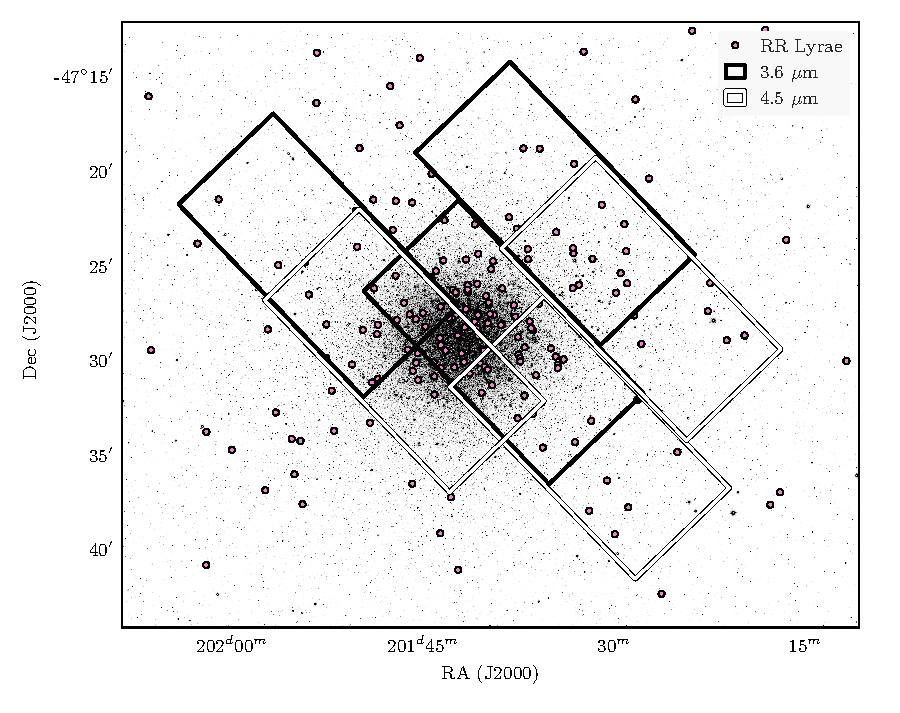
\includegraphics[width=80mm]{final_plots/omegacen_coverage_map.pdf}
\caption{A $K$--band image of $\omega$ Centauri from the FourStar camera, overlaid with the catalog of RR Lyrae \citep{2004A&A...424.1101K} and footprints of the three IRAC fields.}
\label{fig:omegaCen_fields}
\end{center}
\end{figure}


%PSF photometry was performed in PyRAF 2.0 using the \textsc{daophot} package. Initial aperture photometry was performed with an aperture radius of 3.6\arcsec and annulus radius of 4.8\arcsec, whereas the standard IRAC aperture is 6\arcsec; a correction factor of 1.12841 and 1.12738 for 3.6 and 4.5 \micron\ respectively was applied to the instrumental magnitudes. We also calibrate the magnitudes from images in counts (required for \textsc{daophot}) back to flux magnitudes by performing aperture photometry on a set of bright, isolated stars in the flux images, finding the mean difference between the aperture flux magnitudes and PSF counts magnitudes of the same stars, and subtracting said difference from all PSF magnitudes. We also correct for location in the frame using the mosaicked correction images created by \textsc{mopex}

The primary limiting factor in this data is crowding: 77 RR Lyrae variables out of the original catalog of 192 \citet{2004A&A...424.1101K} were rejected due to crowding. To decide which stars to reject we compared the {\it Spitzer} images to a $K$--band image from the FourStar infrared camera on Magellan \citep{2013PASP..125..654P}, with a {\bf resolution of XX arcsec}. This enabled us to see which stars were significantly contaminated and adjust our final sample accordingly. 

{\bf VS NOTE -- I've edited this a little bit, but you need to fill in the resolution of the FourStar image. What you had before was a bit too wordy}. 

\section{Results}
\label{sec:results}
{\bf New section to add --- photometry of all RR Lyrae variables} 
\begin{enumerate}
\item Are you publishing just the IRAC photometry, or the FourStar photometry too?
\item Are you publishing the lightcurves?
\item Need information about how you calculate the average magnitudes for each star
\item Table with cross matched ID's (those from K04), coordinates (always publish RA and Dec so people don't have to go back to another paper, it's really annoying), mags, errs should go here. This is what will get your paper a lot of citations in the future!!
\end{enumerate}

This doesn't need to be a huge section, just a statement of 'this is what my resulting photometry for the RRL was'.

\section{Period--Luminosity Relations}
\label{sec:pl_relation}
\noindent\rule[0.5ex]{\linewidth}{1pt}

{\bf Suggested edits}

Before cutting straight down to the sample that's just stars in all 5 band passes, it would be good to present the whole sample. I suggest that you present the PL relations of the whole sample here, using the theoretical PL relations as reference as you have been doing, but then explain why you want to cut down to the consistent sample.

You also need to be clear about {\bf why} you're fitting the PL relations using only the RRL that appear in all 5 bands. The reason we do this is because when we're fitting a reddening law we want to make sure that there isn't a sampling effect messing up any one (or more) of the uncorrected distance moduli that you're fitting to. If you've got one PL where all the RRL happen to fall at the long P end, or happen to fall brighter than the PL mean for some reason, that's going to mess up your fit. Using a consistent sample reduces that uncertainty. 

\noindent\rule[0.5ex]{\linewidth}{1pt}

Our final RRL sample is comprised of 24 RRL (11 fundamental mode and 13 first overtone) that appear in all five bandpasses. We use the near-- and mid--infrared PL relation parameters presented in {\bf VS CHECK REF FOR BRAGA PAPER} as fiducial in all of our PL fitting. The relations take the form
\begin{equation}M = a + b\times\log P + c\times[Fe/H]\end{equation}
where $a$, $b$, and $c$ are theoretically derived coefficients.
With the use of these coefficients, the distance modulus becomes the only free parameter in our fit. We fit all distance moduli using a weighted least--squares method.

Not all stars in our sample have known metallicity values, thus we use an average [Fe/H] value for all RR Lyrae variables in the cluster. We use both photometric \citep{2000AJ....119.1824R} and spectroscopic \citep{2006ApJ...640L..43S} metallicities for comparison. We find that there is little correspondence between individual metallicity measurements for stars which have both spectroscopic and photometric metallicity values, as shown in Figure~\ref{fig:metallicity_comparison}, and that the average metallicities of the spectroscopic and photometric catalogs differ by nearly 0.1 dex. We use a mean photometric [Fe/H] of  $-1.584$ and a spectroscopic [Fe/H] of $-1.677$.

\begin{figure}
\begin{center}
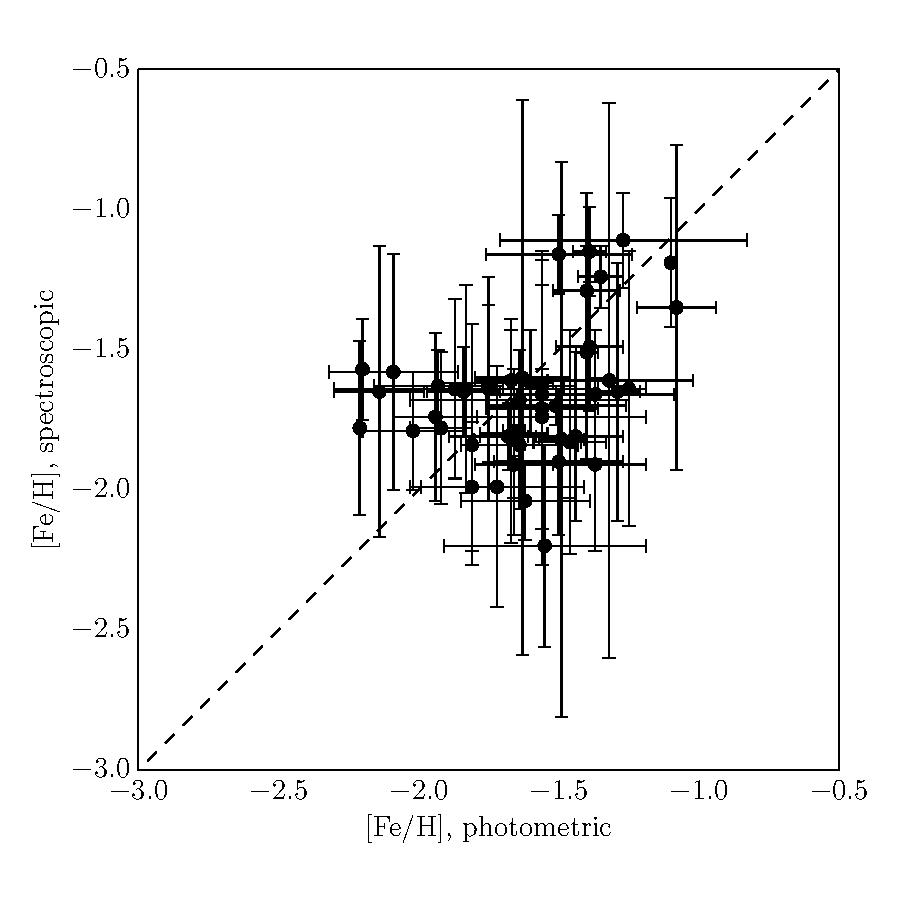
\includegraphics[width=80mm]{final_plots/metallicity_comparison_all.pdf}
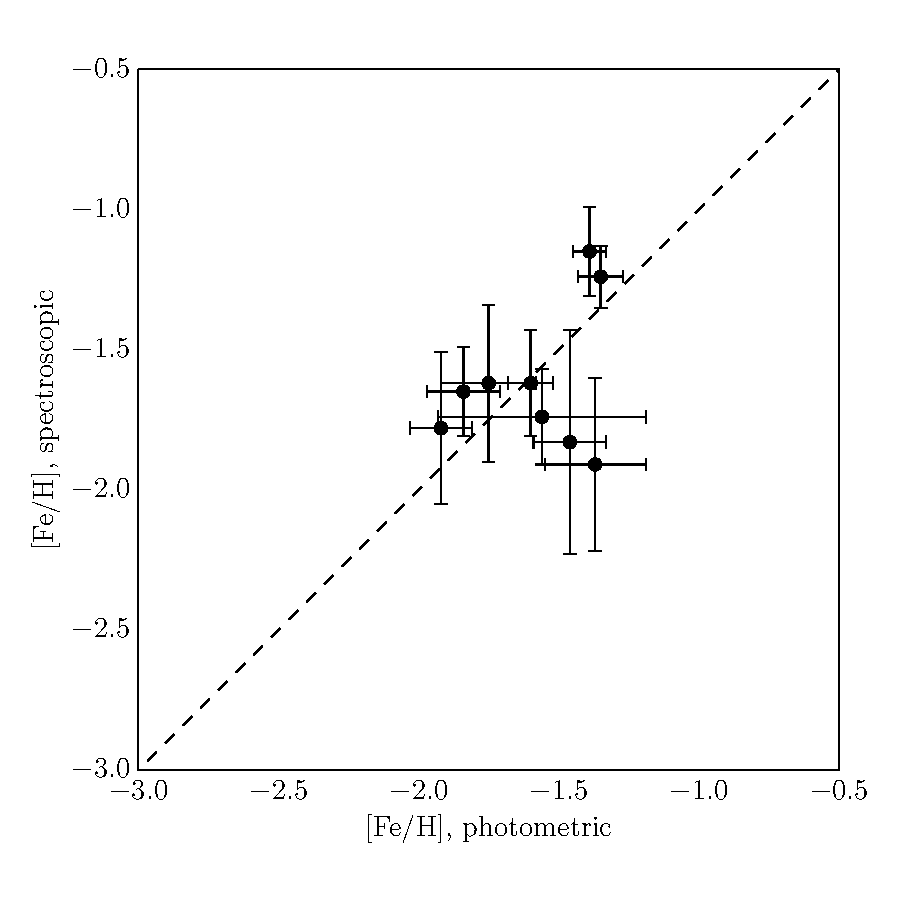
\includegraphics[width=80mm]{final_plots/metallicity_comparison_samestars.pdf}
\caption{Spectroscopic vs. photometric measurements of [Fe/H] for RR Lyrae variables in $\omega$ Centauri. Top: All stars for which both catalogs have [Fe/H] measurements. Bottom: only the stars which appear in our final sample.}
\label{fig:metallicity_comparison}
\end{center}
\end{figure}

The RRL PL relations for each adopted average metallicity are shown in Figures~\ref{fig:omegaCen_pl_spect} and\ref{fig:omegaCen_pl_phot} and described in Table~\ref{tab:pl_table}.

%% Placeholder table for PL relations --- feel free to change the format of this
\begin{table}
\centering
\caption{Mid--IR RR Lyrae period--luminosity relations for $\omega$ Cen.} 
\label{tab:pl_table}
\begin{tabular}{lccccr} 
\hline \hline
Band & [Fe/H] & $a$ & $b$ & $c$ & $\sigma$\\
\hline
[3.6] & $-1.584$ & & & & \\
	& $-1.677$ & & & & \\
[4.5] & $-1.584$ & & & & \\         
	& $-1.677$ & & & & \\
\hline
\end{tabular}
\end{table}

\begin{figure}
\begin{center}
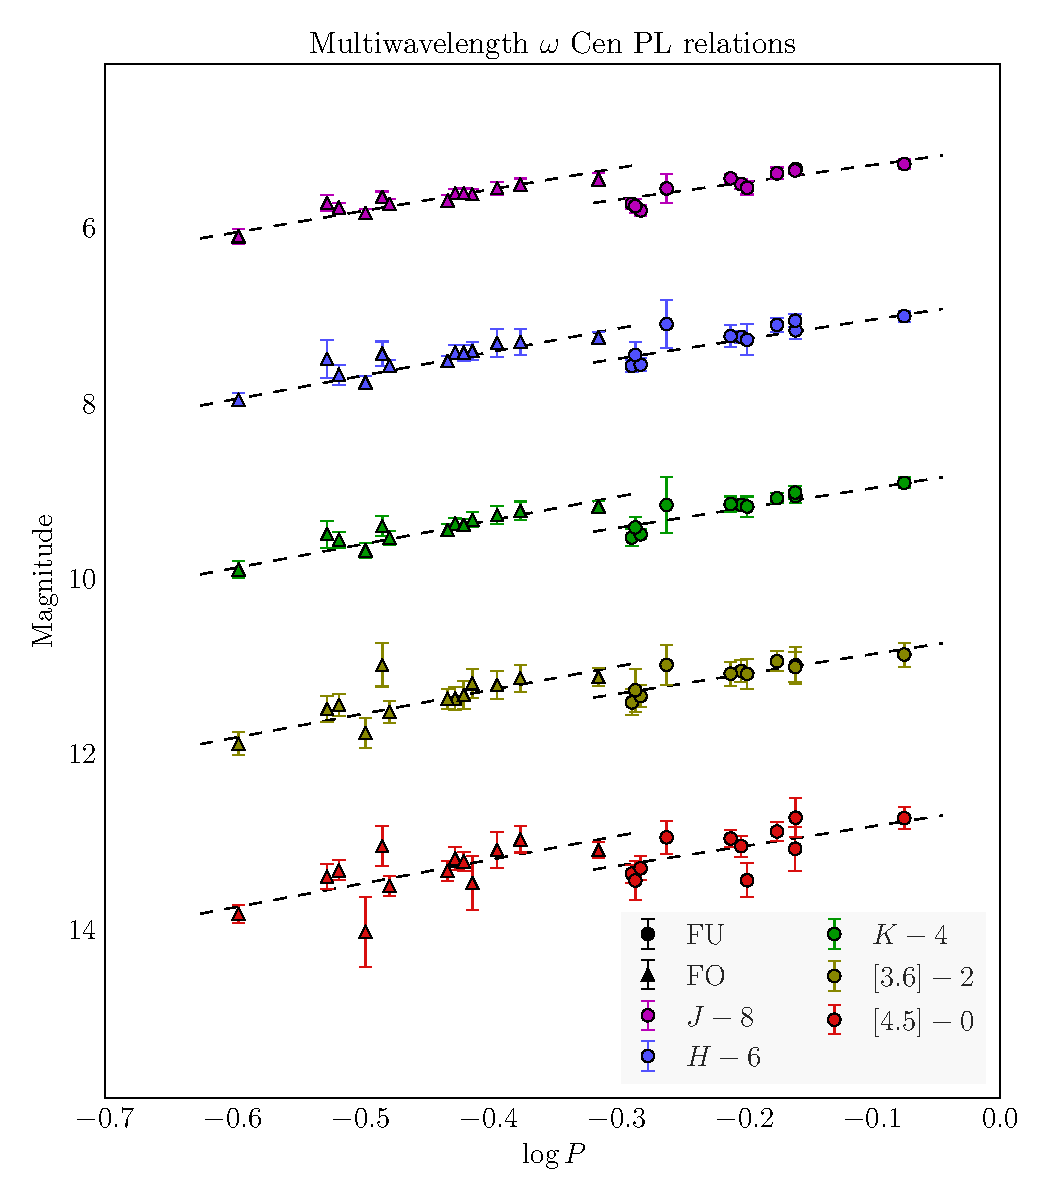
\includegraphics[width=80mm]{final_plots/multiwavelength_PL_samestars_spect.pdf}
\caption{PL relations for $J\!H\!K$, 3.6~$\mu$m, and 4.5~$\mu$m photometry assuming an [Fe/H]$=-1.677$, corresponding to the average  spectroscopic metallicity from \citet{2006ApJ...640L..43S}.  Only those RRL that appear in all five near-- and mid--infrared bands are included in the fit.}
\label{fig:omegaCen_pl_spect}
\end{center}
\end{figure}

\begin{figure}
\begin{center}
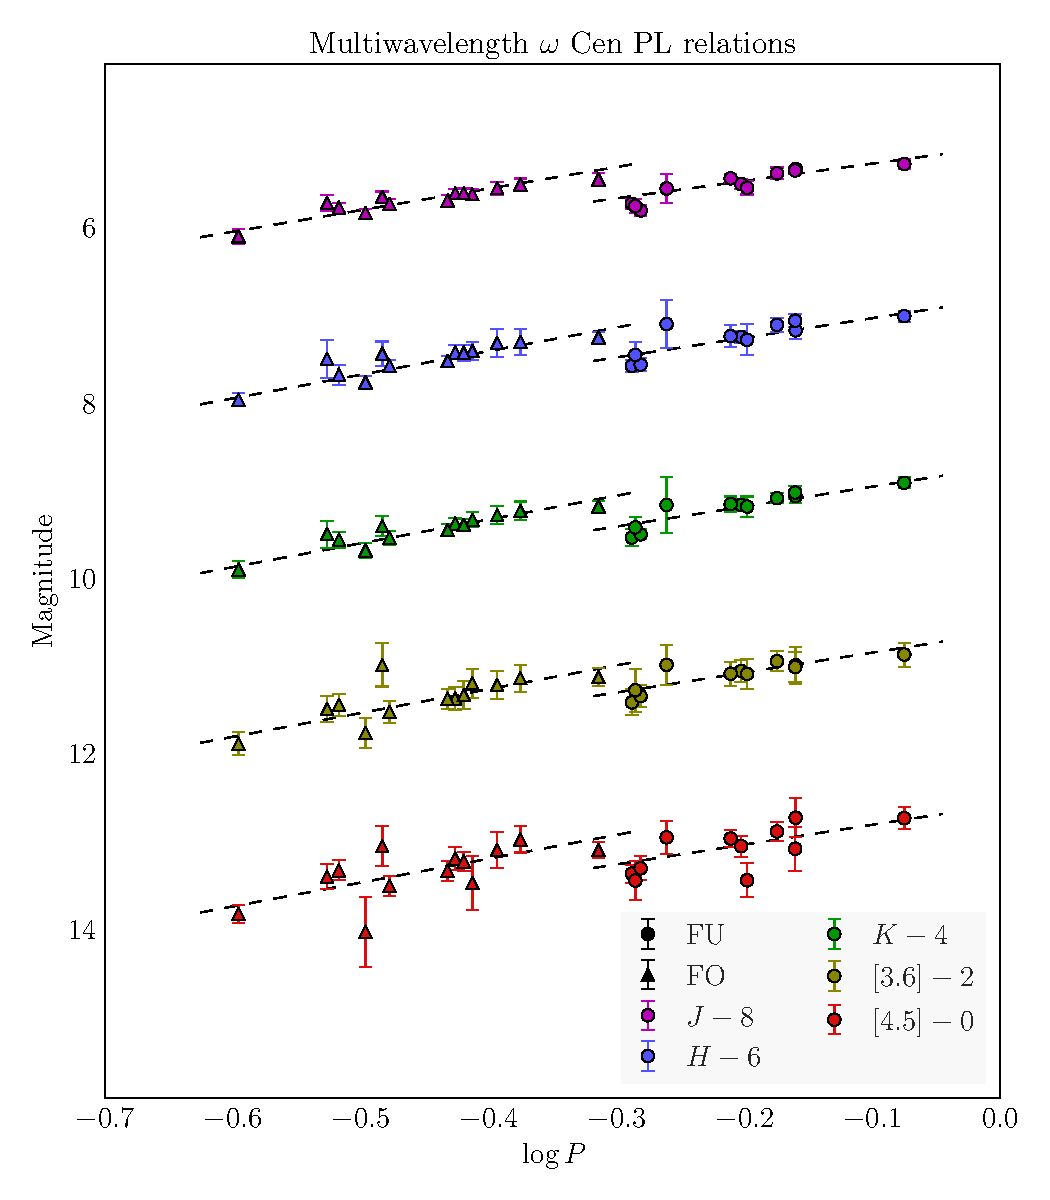
\includegraphics[width=80mm]{final_plots/multiwavelength_PL_samestars_phot.pdf}
\caption{PL relations for $J\!H\!K$, 3.6~$\mu$m, and 4.5~$\mu$m photometry assuming an [Fe/H]$=-1.584$, corresponding to the average photometric metallicity from \citet{2000AJ....119.1824R}. Only those RRL that appear in all five near-- and mid--infrared bands are included in the fit.}
\label{fig:omegaCen_pl_phot}
\end{center}
\end{figure}

\section{Distance Moduli}
\label{sec:distance_moduli}
{\bf The wording on the next paragraph needs changing. It will get caught in the arXiv plagiarism filter right now...}
[Again, shamelessly lifted from the SMC paper]
The five bands for which distance moduli are available can be combined to produce an estimate of the mean $E(B - V)$ and mean reddening--corrected distance modulus of the galaxy. We assume the ratio of total to selective absorption, $R_V = 3.1$, and fit three reddening laws simultaneously. For the near--infrared bands we use the appropriate relation from Cardelli et al. (1989) and for the mid--infrared we use the relation from Indebetouw et al. (2005). The relations are fit by minimising the dispersion of the distance moduli around the values predicted by the reddening law. The resulting fits are shown in Figures~\ref{fig:omegaCen_dist_phot} and \ref{fig:omegaCen_dist_spect}.

\begin{figure}
\begin{center}
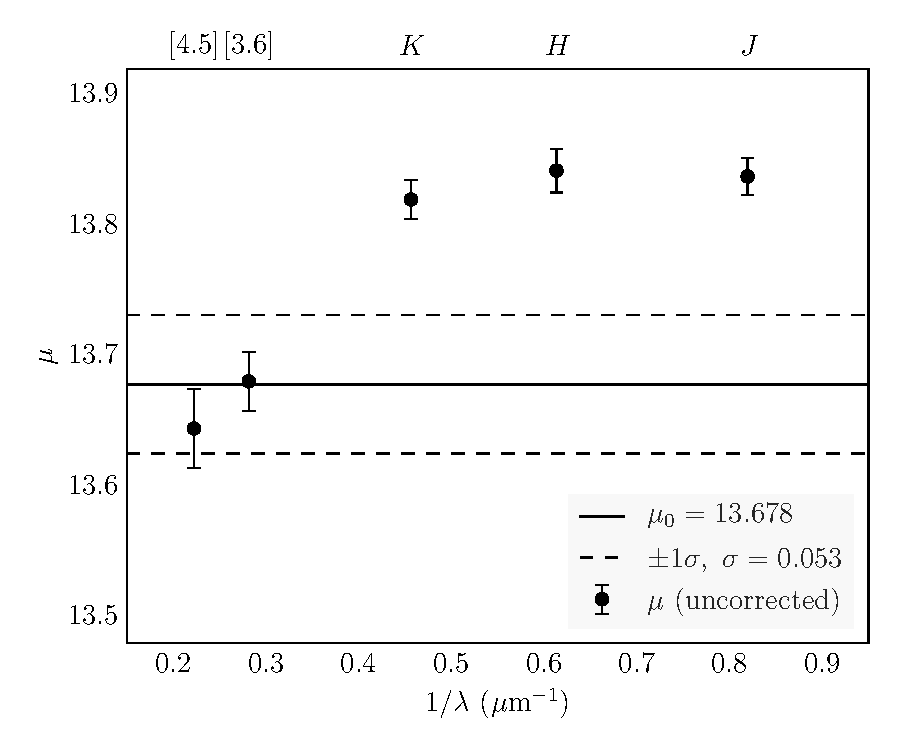
\includegraphics[width=80mm]{final_plots/multiwavelength_distance_samestars_phot.pdf}
\caption{Distance moduli for $J\!H\!K$, 3.6~$\mu$m, and 4.5~$\mu$m photometry using the average photometric metallicity from \citet{2000AJ....119.1824R} {\bf Add the reddening curve to this plot}}
\label{fig:omegaCen_dist_phot}
\end{center}
\end{figure}

\begin{figure}
\begin{center}
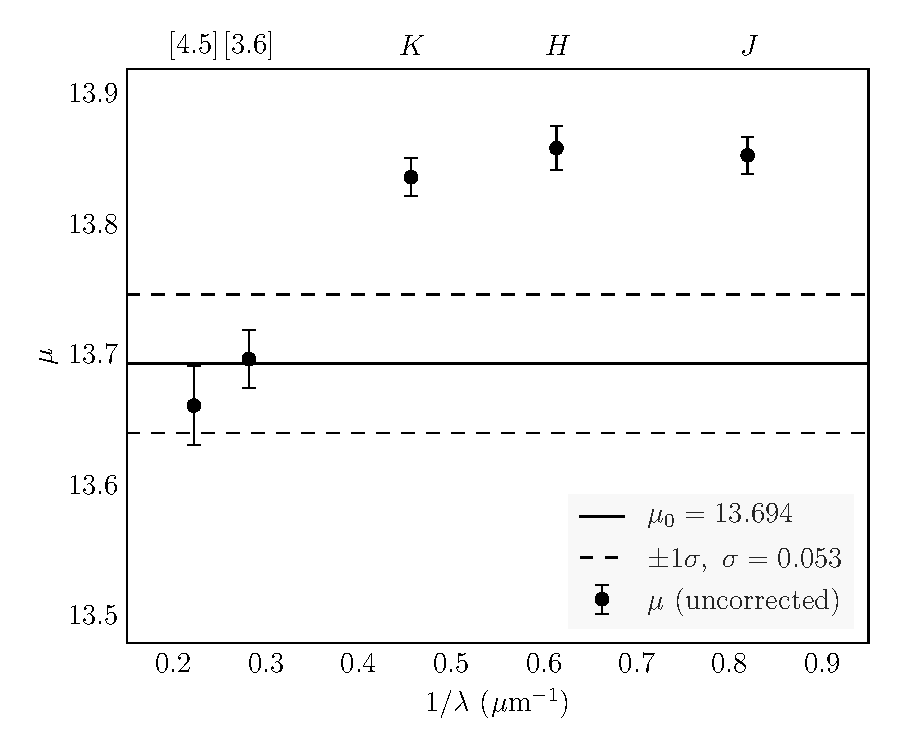
\includegraphics[width=80mm]{final_plots/multiwavelength_distance_samestars_spect.pdf}
\caption{Distance moduli for $J\!H\!K$, 3.6~$\mu$m, and 4.5~$\mu$m photometry using the average spectroscopic metallicity from\citet{2006ApJ...640L..43S} {\bf Add the reddening curve to this plot}}
\label{fig:omegaCen_dist_spect}
\end{center}
\end{figure}


The difference between the distance moduli derived from using spectroscopic and photometric metallicities respectively is less than 0.02 mag, well within the $\pm 0.053$ mag errors for each distance modulus; thus we can say that despite the disagreement between individual metallicity values, for our purposes there is no significant difference between the photometric and spectroscopic metallicity catalogs.

\noindent\rule[0.5ex]{\linewidth}{1pt}
{\bf Suggested edit:} 

Or is it telling you something more fundamental? Like, that the metallicity is having very little effect on the derived distance modulus? That would be a cool thing, right?? Don't sell your science short!!

This isn't definitive evidence but I would suggest something like "the fact that the two distance moduli are indistinguishable is the first hint that the infrared RRL PL relations are not sensitive to metallicity effects". You could repeat something similar at the end of the next paragraph for emphasis, and to lead you into the metallicity section. I would also remove end of the last sentence about "no significant difference between the metallicity catalogues" because I'm not sure that's relevant. 

\noindent\rule[0.5ex]{\linewidth}{1pt}

We find a true mean distance modulus of $\mu_0 = 13.686 \pm 0.053$ [is it cool to just average them], which is in excellent agreement with prior measurements using near--infrared RR Lyrae period--luminosity relations \citep{2006ApJ...652..362D} and and the eclipsing binary OGLEGC17 \citep{2001AJ....121.3089T}, but significantly higher than the distances measured by dynamical modelling \citep{2006A&A...445..513V,
2013MNRAS.436.2598W}

\noindent\rule[0.5ex]{\linewidth}{1pt}
{\bf Suggested edit:} 

I think it's fine just to average them, just make it clear that's what you're doing. You're essentially taking the average metallicity of the two samples by doing this, so you should be clear about that too.

\noindent\rule[0.5ex]{\linewidth}{1pt}

\section{Metallicity}
\label{sec:metallicity}

\noindent\rule[0.5ex]{\linewidth}{1pt}
{\bf Suggested edits:}

You need to step back a bit here. Before going straight into the relations you expect between [Fe/H] and the PL residuals, why do you expect a relation at all? Provide some motivation. They'll be some background in the intro, but not everything. This is where you will flesh it out, and it's OK to repeat things here. 

\begin{enumerate}
\item Why do you expect there to be a metallicity effect? (theory says so is a perfectly good answer, just need to give some refs other than the unpublished PL relations we're using.)
\item Specifically, why do you expect a metallicity effect in the infrared? Here you can discuss the effects we've seen in Cepheids (refer to Monson+ 2012 MW paper (2012ApJ...759..146M), Scowcroft+2011 LMC paper (2011ApJ...743...76S) and Scowcroft+2015 SMC paper (2015arXiv150206995S) where we detect a possible metallicity effect at 4.5um. The metallicity effect in mid-IR Cepheids is proved in Scowcroft et al. 2015, MNRAS, in prep. 
\item Repeat evidence that we do not {\bf expect} a metallicity effect for RR Lyrae 
\begin{itemize}
\item You didn't see a difference in the distance moduli when you used the differnt metallicities
\item You still have a pretty small dispersion in the PL relations {\bf despite crowding}, so any metallicity effect that exists must be smaller than the dispersion in the PL
\end{itemize}
\item Now suggest other ways we could search for a metallicity effect --- correlation between residuals and [Fe/H] for individual stars.
\end{enumerate}

\noindent\rule[0.5ex]{\linewidth}{1pt}

If there is any correlation between [Fe/H] and the PL residuals, we expect it to be a linear one, consistent with the theoretical metallicity terms $c\times[Fe/H]$. We fit a relation of the form
\begin{equation}\Delta[\lambda] = c\times[Fe/H] + d\end{equation}
to the 3.6~$\mu$m and 4.5~$\mu$m PL residuals and metallicity values for stars with individual metallicity values, as shown in Figures~\ref{fig:delta_3p6_phot}, \ref{fig:delta_3p6_spect}, \ref{fig:delta_4p5_phot}, and \ref{fig:delta_4p5_spect}. Relations were fit without weighting individual errors in either $\Delta[\lambda]$ or [Fe/H]. Although there are relatively large errors in both variables, they are consistent enough that weighting by errors would result in a fit heavily skewed by the few data points with low errors.

\begin{figure}
\begin{center}
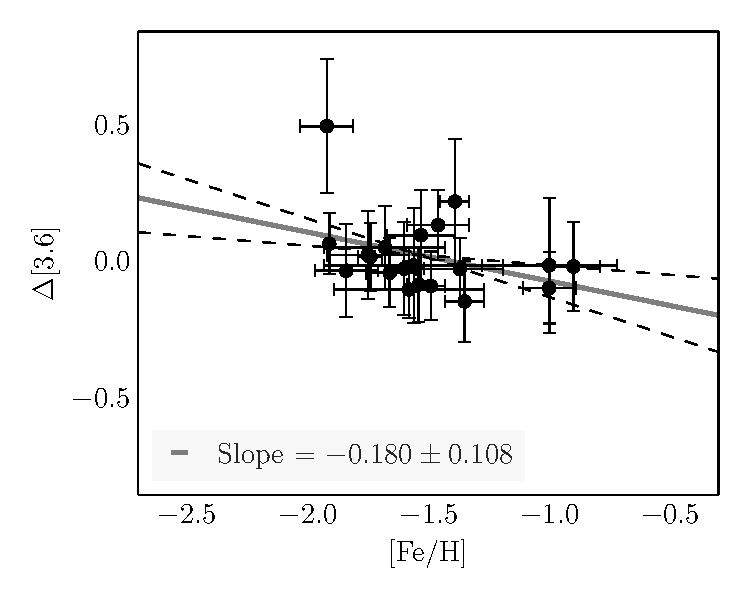
\includegraphics[width=80mm]{final_plots/delta_feh_3p6_phot.pdf}
\caption{[Fe/H] vs. $\Delta$~3.6~$\mu$m using photometric metallicities}
\label{fig:delta_3p6_phot}
\end{center}
\end{figure}


\begin{figure}
\begin{center}
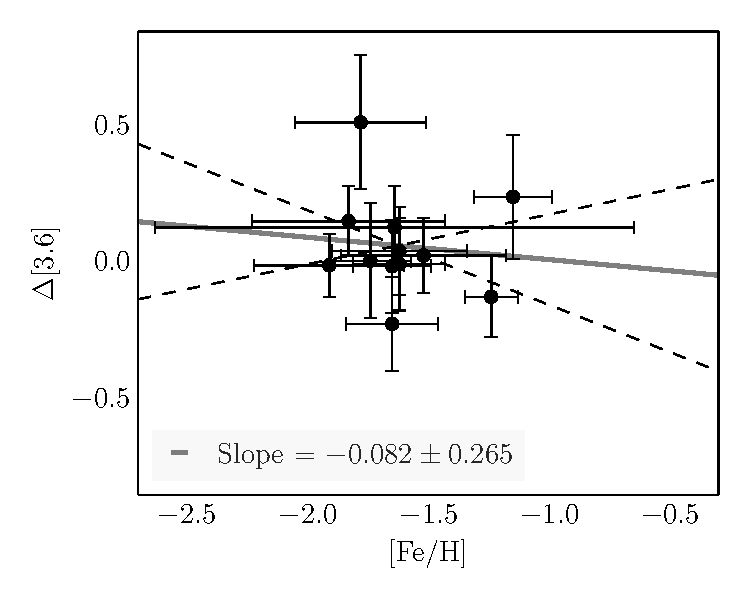
\includegraphics[width=80mm]{final_plots/delta_feh_3p6_spect.pdf}
\caption{[Fe/H] vs. $\Delta$~3.6~$\mu$m using spectroscopic metallicities}
\label{fig:delta_3p6_spect}
\end{center}
\end{figure}

\begin{figure}
\begin{center}
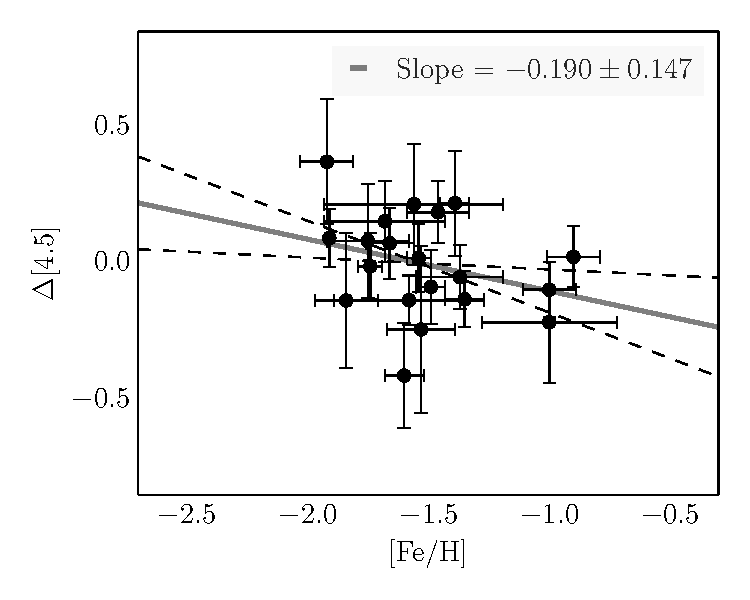
\includegraphics[width=80mm]{final_plots/delta_feh_4p5_phot.pdf}
\caption{[Fe/H] vs. $\Delta$4.5~$\mu$m using photometric metallicities}
\label{fig:delta_4p5_phot}
\end{center}
\end{figure}

\begin{figure}
\begin{center}
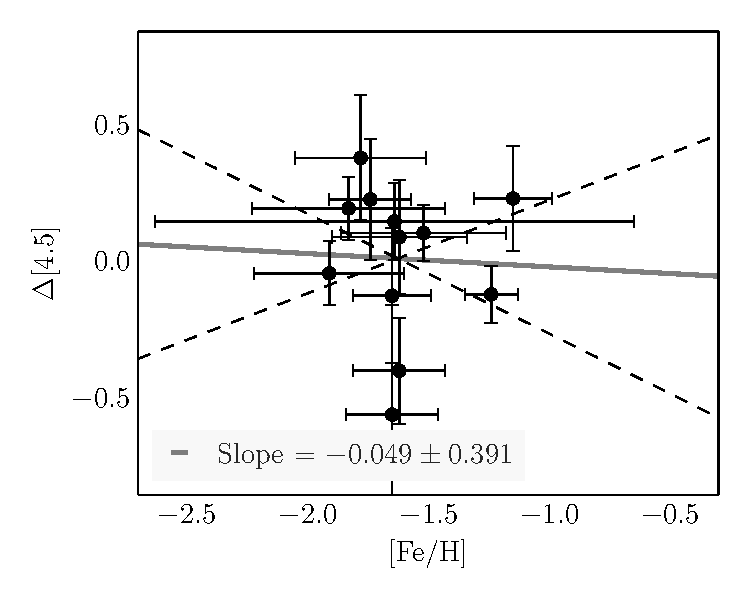
\includegraphics[width=80mm]{final_plots/delta_feh_4p5_spect.pdf}
\caption{[Fe/H] vs. $\Delta$4.5~$\mu$m using spectroscopic metallicities}
\label{fig:delta_4p5_spect}
\end{center}
\end{figure}


\section{Discussion}
\label{sec:discussion}

{\bf This section we can work on once you've worked on the others. I think it will write a lot of itself after you've done the other bits.}

We find that although the scatter in the 3.6~$\mu$m and 4.5~$\mu$m PL relations is higher for $\omega$ Centauri than it is for M4 \citep{2015arXiv150507858N}, there is no evidence that it is due to metallicity. When we fit a line to [Fe/H] vs. $\Delta$3.6~$\mu$m and $\Delta$4.5~$\mu$m, both slopes are within $2\sigma$ of zero, indicating that there is no significant metallicity dependence in the PL residuals. When the outlier in [Fe/H] vs. 3.6~$\mu$m at [Fe/H] = $-2.0$ is removed from the photometric metallicities, the slopes of [Fe/H] vs. 3.6~$\mu$m and 4.5~$\mu$m both move within $1\sigma$ of zero.

Alternative explanations for the increased scatter relative to M4 include crowding and [other things here].


\section{Conclusions}
\label{sec:conclusions}


\section*{Acknowledgements}
\label{sec:acknowledgements}

We thank Eric Persson for his many contributions to this project.

This work is based on observations made with the Spitzer Space Telescope, which is operated by the Jet Propulsion Laboratory, California Institute of Technology under a contract with NASA. Support for this work was provided by NASA through an award issued by JPL/Caltech.


%%%%%%%%%%%%%%%%%%%%%%%%%%%%%%%%%%%%%%%%%%%%%%%%%%

%%%%%%%%%%%%%%%%%%%% REFERENCES %%%%%%%%%%%%%%%%%%

% The best way to enter references is to use BibTeX:

\bibliographystyle{mnras}
\bibliography{omegaCen_mnras_2015}
 % if your bibtex file is called example.bib


% Alternatively you could enter them by hand, like this:
% This method is tedious and prone to error if you have lots of references

%%%%%%%%%%%%%%%%%%%%%%%%%%%%%%%%%%%%%%%%%%%%%%%%%%

%%%%%%%%%%%%%%%%% APPENDICES %%%%%%%%%%%%%%%%%%%%%


\begin{figure}
\begin{center}
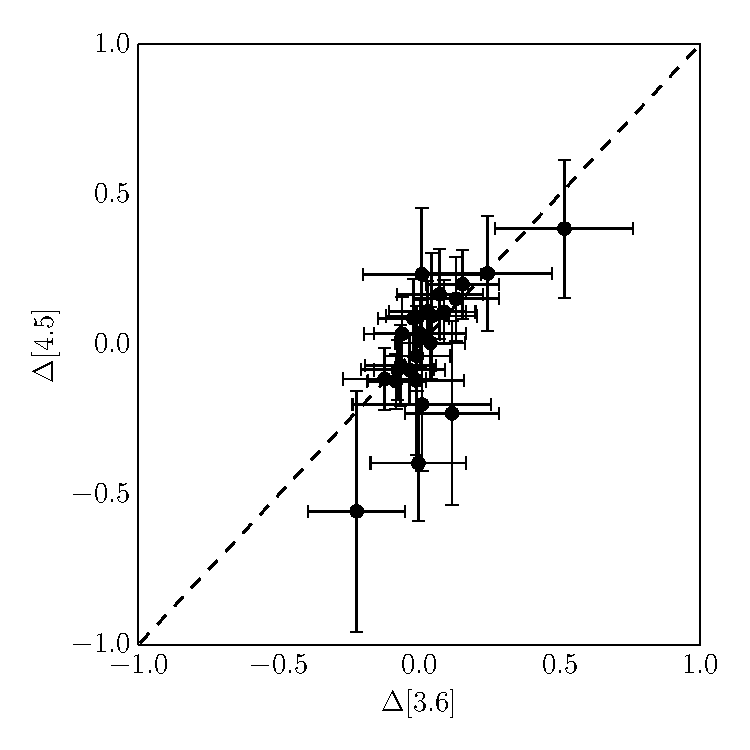
\includegraphics[width=80mm]{final_plots/deltadelta_3p6_4p5_spect.pdf}
\caption{$\Delta$~3.6~$\mu$m vs. $\Delta$~4.5~$\mu$m using spectroscopic metallicities}
\label{fig:deltadelta_spect}
\end{center}
\end{figure}



\begin{figure}
\begin{center}
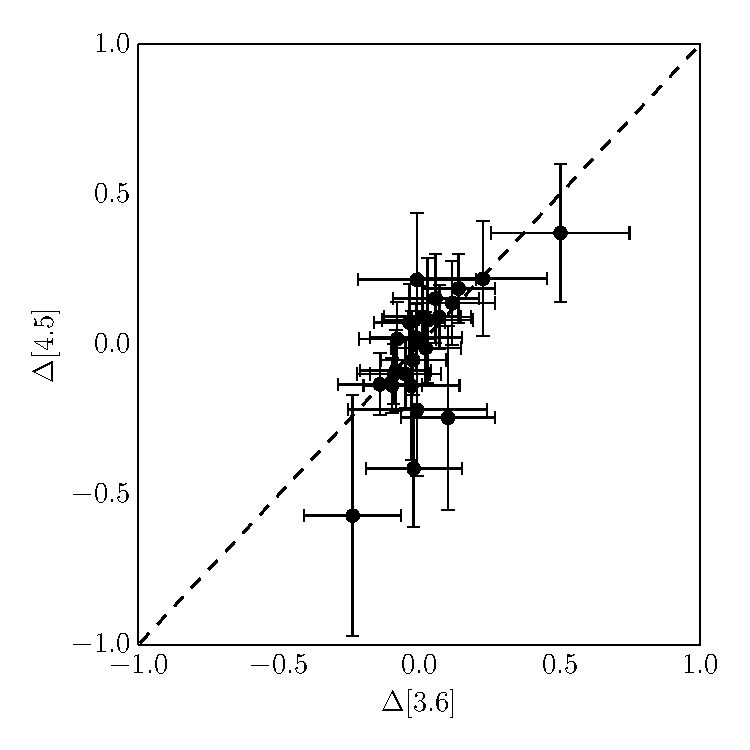
\includegraphics[width=80mm]{final_plots/deltadelta_3p6_4p5_phot.pdf}
\caption{$\Delta$~3.6~$\mu$m vs. $\Delta$~4.5~$\mu$m using photometric metallicities}
\label{fig:deltadelta_phot}
\end{center}
\end{figure}



%%%%%%%%%%%%%%%%%%%%%%%%%%%%%%%%%%%%%%%%%%%%%%%%%%


% Don't change these lines
\bsp	% typesetting comment
\label{lastpage}
\end{document}

% End of mnras_template.tex